В работах \cite{Thompson,Tong} описан устойчивый итерационный алгоритм эволюции поверхностной сетки, сохраняющий целевой объем льда.
В нем используется ряд улучшений по сравнению с классическими методами.

Многослойный подход, реализованный в этом методе, не использует константное количество шагов - величина наращиваемого объема на каждом шаге алгоритма рассчитывается исходя из максимально допустимой доли временного шага обледенения, после превышения которого возможно развитие численной нестабильности в эволюции поверхности.
Наиболее очевидный случай возникает, когда проекции нормалей граней пересекаются, в этом случае слишком большой временной шаг приведет к складыванию поверхности.
Чтобы идентифицировать грани, которые будут демонстрировать подобное поведение на текущем временном шаге, предполагается, что объем, образованный путем вытягивания треугольной грани с использованием параллельной плоскости смещения, образует призматоид, объем которого определяется кубической функцией высоты $h$:

\begin{equation}\label{Tong:1}
V(h)=ah+bh^2+ch^3
\end{equation}

где константы $a$, $b$, $c$ определяются позициями узлов грани, их нормалей и нормалью грани.
Рассмотрим корни квадратного уравнения, которое получается в результате дифференцирования уравнения \ref{Tong:1}.
Если корни являются положительными вещественными значениями, наименьший положительный корень определяет высоту, на которой достигается максимальный объем, которая обозначается как $V_{max}$, иначе функция монотонна с возрастанием и ограничение на шаг в данной грани не требуется.
Исходя из этого, можно вычислить максимальную долю временного шага обледенения, которая требуется для обеспечения разумного поведения накопления объема.
В дополнение к этому пределу размера шага был введен предел стабильности $\alpha_{jiao}$, который основан на том, как изменяются направления нормалей по мере эволюции поверхности \cite{Jiao}.
Тогда, допустимая доля временного шага для $i$-й грани определяется как

\begin{equation}\label{Tong:2}
\alpha_{\Delta t}^i=
\begin{cases}
min(s_{\Delta t}\frac{V_{max}^i}{V_f},\alpha_{jiao},1), \text{if $V_{max}^i$ exists}, \\
\alpha_{jiao}, \text{if $V_{max}^i$ doesn't exist}
\end{cases}
\end{equation}

где $s_{\Delta t}$ ($0 < s_{\Delta t} < 1$) -- эмпирически определяемый коэффициент, $V_f$ -- текущий оставшийся объем приращения льда для $i$-й грани.
Тогда объем, наращенный для текущего шага, равен $\alpha_{\Delta t} V_f$, где $\alpha_{\Delta t}$ представляет собой глобальное минимальное значение для всех граней.

Другой важной особенностью алгоритма является введение первичного и нулевого простанств, описанных в \cite{Jiao_null_space_smooth}.
Если эволюционное движение узлов сетки происходит в первичном пространстве, то их перемещение в нулевом пространстве будет сохранять потенциальную точность второго порядка триангуляции поверхности, благодаря чему мы можем  проводить сглаживание поверхности сетки с сохранением объема.
В алгоритме используется несколько видов сглаживаний.

Первое сглаживание -- сглаживание нормалей в вершинах и ячейках сетки.
Чтобы сделать возможным сглаживание в нулевом пространстве, все нормали в узлах рассчитываются так, чтобы они лежали в первичном пространстве, а перемещение узлов при наращивании льда происходит только по их нормалям.
По мере эволюции, на поверхности может усиливаться шум -- если его не контролировать, может возникнуть ситуация, когда двугранный угол между гранями станет слишком малым и ограничит максимальную долю временного шага обледенения.
Для уменьшения поверхностного шума, перед наращиванием льда применяется локальное сглаживание, регулирующее направление смещения узла в проблемных областях, чтобы оно более точно совпадало с направлениями его соседей.
Этот метод может улучшить гладкость поверхности в некоторых ситуациях.
Основная цель сглаживания нормалей -— вытолкнуть точки из вогнутых областей, где нормали могут локально сходиться.
Сглаживание нормалей достигается с помощью серий взвешенных средних, которые предназначены для придания веса нормалям, генерируемым проблемными областями.

Второе сглаживание -- сглаживание высот.
После вычисления доли временного шага и объема, наращиваемого для текущего шага, для эволюции поверхности необходимо определить поле высот, которое будет соответствовать этому объему, чтобы по нему определить смещения узлов сетки.
Решение $V(h_i) = \alpha_{\Delta t} V_f$ обеспечивает поле начальных высот, которое используется для движения поверхности.
Цель дополнительного шага сглаживания высоты состоит в том, чтобы отфильтровать высокочастотный шум в поле высот за счет уменьшения разницы высот между соседними гранями.
Как правило, высоты двух треугольных граней, имеющих общее ребро, не будут равными.
На данном шаге используется сглаживание высот с сохранением объема путем его перераспределения между соседними гранями.

\begin{figure}
  \centering
  \begin{minipage}[h]{0.49\textwidth}
    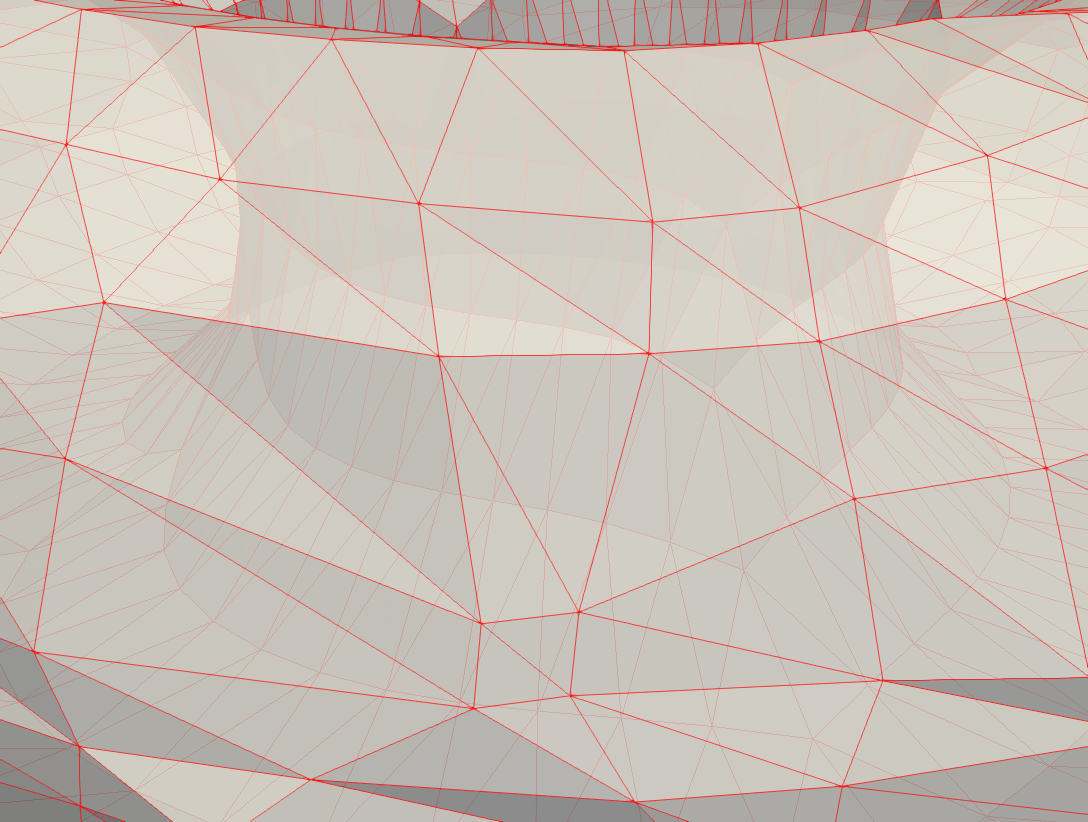
\includegraphics[width=\textwidth]{pics/pic_smooth_before.png}
    \caption{Mesh before null-space smoothing}\label{fig:pic_smooth_before}
  \end{minipage}
  \hfill
  \begin{minipage}[h]{0.49\textwidth}
    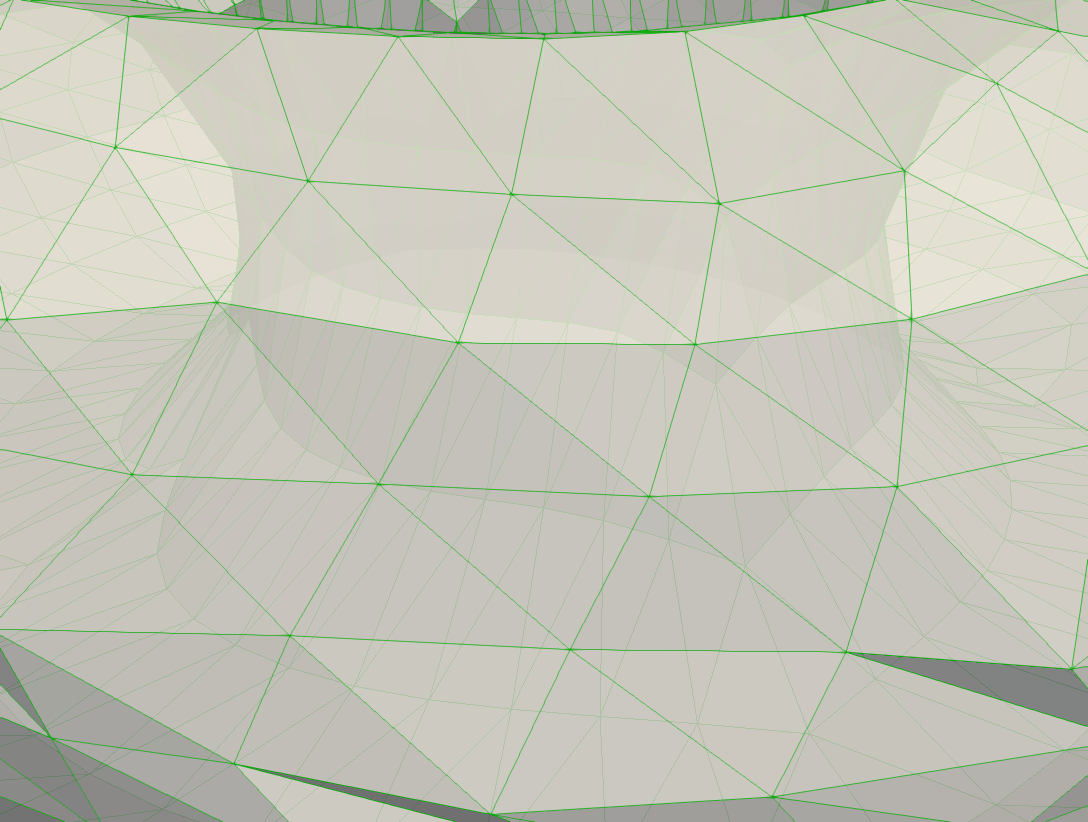
\includegraphics[width=\textwidth]{pics/pic_smooth_after.png}
    \caption{Mesh after null-space smoothing.}\label{fig:pic_smooth_after}
  \end{minipage}
\end{figure}

Последним типом сглаживания является сглаживание в нулевом пространстве.
Эволюция поверхности будет стремиться упаковать узлы в вогнутые области, где сходятся нормали к поверхности, тогда как расширение сетки происходит в выпуклых областях, где нормали к поверхности расходятся.
Если узлы не будут перераспределены, может стать невозможным продолжать продуктивный, стабильный временной шаг.
Для улучшения качества поверхностной сетки узлы перераспределяются на поверхности с помощью сглаживания в нулевом пространстве.
Этот метод способен перераспределять точки, сохраняя при этом целостность базовой геометрии.
Нулевое пространство определяется касательной плоскостью (для гладких областей), касательной линией (для складок поверхности) или пустым пространством (для углов), движущиеся в нем узлы остаются на поверхности, так что объем и форма поверхности могут быть сохранены (Fig.~\ref{fig:pic_smooth_before}, Fig.~\ref{fig:pic_smooth_after}).